% %
%


\documentclass{article}
\usepackage{pgfplots}

\usepackage{graphicx}
\usepackage{amssymb}
\usepackage{amsmath}
\usepackage{epstopdf}
\usepackage{enumerate}
\usepackage{multirow}
\usepackage[usenames,dvipsnames,svgnames,table]{xcolor}
\usepackage{url}
\usepackage{dirtree}
\usepackage{capt-of}
\usepackage{multicol}
\usepackage[hidelinks]{hyperref}
\usepackage{subcaption}
\usepackage{listings}
\usepackage{xcolor}
\usepackage{tcolorbox}
\tcbuselibrary{skins,breakable}
\usepackage{booktabs}
\definecolor{codegreen}{rgb}{0,0.6,0}
\definecolor{codegray}{rgb}{0.5,0.5,0.5}
\definecolor{codepurple}{rgb}{0.58,0,0.82}
\definecolor{backcolour}{rgb}{0.95,0.95,0.92}


\lstdefinestyle{mystyle}{
    backgroundcolor=\color{backcolour},   
    commentstyle=\color{codegreen},
    keywordstyle=\color{magenta},
    numberstyle=\tiny\color{codegray},
    stringstyle=\color{codepurple},
    basicstyle=\ttfamily\footnotesize,
    breakatwhitespace=false,         
    breaklines=true,                 
    captionpos=b,                    
    keepspaces=true,                 
    numbers=left,                    
    numbersep=5pt,                  
    showspaces=false,                
    showstringspaces=false,
    showtabs=false,                  
    tabsize=2
}

\lstset{style=mystyle}

\newcommand{\class}{ CS37300 }
% \newcommand{\website}{{\tiny\url{https://www.cs.purdue.edu/homes/smith/courses/Fall2022}}}
\newcommand{\homeworknumber}{3}
% \newcommand{\duedate}{Feb 14, 2023 (6pm) }

\setlength{\parskip}{1pc}
\setlength{\parindent}{0pt}
\setlength{\topmargin}{-3pc}
\setlength{\textheight}{9.5in}
\setlength{\oddsidemargin}{0pc}
\setlength{\evensidemargin}{0pc}
\setlength{\textwidth}{6.5in}

\newcommand{\var}{\mbox{var}}
\newcommand{\cov}{\mbox{cov}}

\newcommand{\newpart}{
\stepcounter{partno}
\noindent
{\bf (\alph{partno})}
}

\newcommand{\header}{
\newpage
\noindent
\framebox{ \vbox{\class Homework \hfill --- Homework \homeworknumber --- \hfill  Last update: Oct 5, 2026
  \\ \hfill {\color{red} Theory Due Date: Oct 19, 2026 (11:59 pm)}\\{\color{red} Programming Due Date: Oct 26, 2026 (11:59 pm)} }}
\bigskip

Name: \rule[-3pt]{7cm}{0.05em} \ \ \ \ PUID: \rule[-3pt]{7cm}{0.05em}

{\bf Instructions and Policy:} 
You are allowed to study with others and use online resources for reference, however, the work you turn in must be your own. This means do not copy/paste from Stack Exchange (or from another student.) If you have worked closely with other students, provide their name(s) and a brief (at most one paragraph) description of the interaction; if we feel this oversteps the bounds, we will discuss it with you. Each student should write up their own solutions independently.

The requirements below are supposed to be followed in this and further homework assignments.

\begin{itemize}
\item For your theoretical submission:
    \begin{itemize}
    \item {\color{red} YOU MUST INCLUDE YOUR NAME IN THE HOMEWORK.}
    \item The answers {\color{red} MUST be submitted via Gradescope under HW3-Theory}. 
    \item Please write clearly and concisely - clarity and brevity will be rewarded. Refer to known facts as necessary. 
    \item Theoretical questions {\color{red} MUST include the intermediate steps to the final answer}.
    \end{itemize}
\item For your programming answers:
    \begin{itemize}
        \item {\color{red} The Python scripts should be submitted separately via Gradescope under HW3-programming}
        \item Zero points will be given in any question where the Python code answer doesn't match the answer on Gradescope.
    \end{itemize}
\end{itemize}



Your code is REQUIRED to run on Python 3.11 in an environment detailed in Homework 0 under the Python Installation section. While your code may run in other environments, any points lost due to environmental issues will not be regraded.

Please make sure you don't use any libraries that are not imported for you. If such a library is used, you will get 0 pt for the coding part of the assignment.

If your code doesn't run on Gradescope, then even if it compiles on another computer, it will still be considered not running and the respective part of the assignment will receive 0 pt.
}



\newcounter{questionno}
\setcounter{questionno}{0}
\newcounter{partno}

\newcommand{\question}[1]{
\noindent
\newline
\stepcounter{questionno}
\setcounter{partno}{0}
{\bf \large Q\arabic{questionno} (#1 pts): }
}

\begin{document}

\header


\newpage

\question{{\color{red}0pts correct answer,  -1,000pts incorrect answer: (0,-1,000)}} 
A correct answer to the following questions is worth 0pts. An incorrect answer is worth -1,000pts, which carries over to  other homeworks and exams, and can result in an F grade in the course.
\begin{enumerate}[(1)]
\item Student interaction with other students / individuals:
\begin{enumerate}[(a)]
\item I have copied part of my homework from another student or another person (plagiarism).
\item Yes, I discussed the homework with another person but came up with my own answers. Their name(s) is (are) \_\_\_\_\_\_\_\_\_\_\_\_\_\_\_\_\_\_\_\_\_\_\_\_\_\_\_\_\_\_\_\_\_\_\_\_\_\_\_\_\_\_\_\_ 
\item No, I did not discuss the homework with anyone
\end{enumerate}
\item On using online resources:
\begin{enumerate}[(a)]
\item I have copied one of my answers directly from a website (plagiarism).
\item I have used online resources to help me answer this question, but I came up with my own answers (you are allowed to use online resources as long as the answer is your own). Here is a list of the websites I have used in this homework:\\\_\_\_\_\_\_\_\_\_\_\_\_\_\_\_\_\_\_\_\_\_\_\_\_\_\_\_\_\_\_\_\_\_\_\_\_\_\_\_\_\_\_\_\_\_\_\_\_\_\_\_\_\_\_\_\_\_\_\_\_\_\_\_\_\_\_\_\_\_\_\_\_\_\_\_\_\_\_\_\_\_\_\_\_\_\_\_\_ 
\item I have not used any online resources except the ones provided in the course website.
\end{enumerate}


\end{enumerate}

\newpage
\section*{Theoretical Questions (12+20+16+15+12= 75 pts)}

{\bf Please submit your answers on Gradescope.}

\question{12} {\bf \large True or False questions}
\paragraph{Answer the following as True or False with a justification or example. Points are uniformly distributed within the questions.}~

\begin{enumerate}[(a)]
\item ({\bf 4 pts}) Due to the EM algorithm's iterative process, it will always converge to a global maximum of the likelihood.
\begin{tcolorbox}[breakable,
enhanced,
notitle,
width=16.1cm,
height=3cm]
%
% Your solution here
%
 {
     }

\end{tcolorbox}

\item ({\bf 4 pts}) 

For a linearly separable dataset, when applying a soft-margin SVM the hyperplane is always the same as hard-margin SVM regardless of the regularization parameter.

\begin{tcolorbox}[breakable,
enhanced,
notitle,
width=16.1cm,
height=3cm]
%
% Your solution here
%
 { }

\end{tcolorbox}

\item ({\bf 4 pts}) 
The gradient descent algorithm always finds the global minimum. 

\begin{tcolorbox}[breakable,
enhanced,
notitle,
width=16.1cm,
height=3cm]
%
% Your solution here
%
 {}


\end{tcolorbox}
\end{enumerate}

\newpage

\question{20} {\bf \large Cross-validation}

\begin{figure}[bth]
    \centering
    \begin{subfigure}[b]{0.49\textwidth}
        \centering
        \includegraphics[width=0.95\linewidth]{25Spring/HW3/figures/m1.png}
        \caption{Training and validation loss of a model $M_1$}
        \label{fig:m2}
    \end{subfigure}
    \centering
    \begin{subfigure}[b]{0.49\textwidth}
        \centering
        \includegraphics[width=\linewidth]{25Spring/HW3/figures/m2.png}
        \caption{Training and validation loss of a model $M_2$}
        \label{fig:m1}
    \end{subfigure}
    \caption{Example of training curves showing training and validation loss for two hypothetical models $M_1$ and $M_2$.}
\end{figure}

\begin{enumerate}
[1.]
\item \textbf{(6 pts)} Review the training and validation loss curve in Figure~\ref{fig:m1} (model $M_2$).
The $y$-axis shows a loss (lower is better) for the training and validation data.
The $x$-axis shows the iterations to update the model parameters (e.g. update steps on Perceptron algorithm or steps of gradient descent for logistic regression).\\
{\bf Hint:} Note that these are training curves, not learning curves.



\begin{enumerate}

\item {(\bf 3 pts)} Are the best parameters for model $M_2$ at 100 iterations or at 400 iterations? Please justify your answer.

\begin{tcolorbox}[breakable,
enhanced,
notitle,
width=14.5cm,
height=2cm]
{
}
%

\end{tcolorbox}
\item {(\bf 3 pts)} What is the disadvantage of choosing the model with parameters obtained at 50 iterations?

\begin{tcolorbox}[breakable,
enhanced,
notitle,
width=14.5cm,
height=2cm]
%
{
}
%
\end{tcolorbox}
\end{enumerate}

% ---- %
\newpage
\item \textbf{(4 pts)} Review the training and validation loss curve in Figure~\ref{fig:m2} of model $M_1$. 

Which of the following explanations and decisions are appropriate for the observed behavior in \ref{fig:m2}?\\
{\bf Select all TRUE statements. No justification is necessary.}
\begin{enumerate}[(A)]
    \item The validation data is scarce and not very representative.
    \item The training data does not provide sufficient information to learn the problem relative to the validation data used to evaluate it.
    \item Getting more validation data will not reduce the training loss.
    \item The training loss has converged, so obtaining more and better training data will not reduce the training loss further.
\end{enumerate}

%\begin{tcolorbox}[breakable,
%enhanced,
%notitle,
%width=15.1cm,
%height=5cm]
%
% Your solution here
% tutorial data example change
%
 {}

%\end{tcolorbox}

\item \textbf{(4 pts)} Which statements about $k$-fold cross-validation are correct?\\
{\bf Select all TRUE statements. No justification is necessary.}
\begin{enumerate}[(A)]
    \item When using $k$-fold cross-validation, using a smaller $k$ means it will take more time to run the evaluation.
    \item With a larger $k$, the training set gets larger, while the test set gets smaller.
    \item When splitting data into folds, it is desirable to minimize the variance across folds.  
    \item When $k=N$, where $N$ is the size of the data set, $k$-fold cross-validation is not the same as leave-one-out cross-validation.
    \item None of the above
\end{enumerate}

%\begin{tcolorbox}[breakable,
%enhanced,
%notitle,
%width=15.1cm,
%height=5cm]
%
% Your solution here
%

 {}
%\end{tcolorbox}

\newpage
\newpage
\item \textbf{(6 pts)} Given the supervised learning dataset with 3 training examples $(X_1,Y_1) =(-2,-1)$, $(X_2,Y_2)=(-1,-1)$, $(X_3,Y_3) = (0,1)$, use the Perceptron algorithm to learn a classifier. If needed, use $\text{sign}(0)=1$.  The Perceptron classifier will have two parameters $w=(w_0, w_1)$ (the first parameter, $w_0$ acts as the bias).
What is the average 0-1 loss of the Perceptron algorithm evaluated by 3-fold cross-validation? (Please also describe, for each fold/iteration of the cross-validation, what is the training data used and the loss obtained).


\begin{tcolorbox}[breakable,
enhanced,
notitle,
width=15.5cm,
height=18cm]
{
}
\end{tcolorbox}
\end{enumerate}






\newpage
\question{16} {\bf \large SVM}

Consider an SVM that obtains a linear decision boundary through finding a hyperplane indexed by $(\hat{\textbf{w}},\hat{b})$ that is consistent with the training examples while maximizing the margin with respect to the training examples as described in Equation (\ref{eq:hard_svm}), which is equivalent to the quadratic optimization problem described in Equation (\ref{eq:hard_svm_min}), where $(\textbf{w},b)$ denote the parameters of the hyperplane, $x_i$ the $i$-th training example, $y_i \in \{-1, 1\}$ the class label for the $i$-th training example, $N$ the number of instances.


\begin{equation}
\begin{aligned}
\label{eq:hard_svm}
% &\max _{\beta, \beta_0,\|\beta\|_{2}=1} M \\
% \text{subject to   }\text{  } y_i&\left(x_i^T \beta+\beta_0\right) \geq M,\; i=1, \ldots, N.
(\hat{\textbf{w}},\hat{b}) = \arg\max_{(\textbf{w},b):\|\textbf{w}\| = 1} \min_{1\leq i \leq n} y_i(\textbf{w}^Tx_i +b)
\end{aligned}
\end{equation}


which is equivalent to


\begin{equation}
\label{eq:hard_svm_min}
\begin{aligned}
&\min _{\textbf{w},b} \frac{1}{2}\|\textbf{w}\|_{2}^2\\
\text{subject to   }\text{  }   & y_i(\textbf{w}^Tx_i +b) \geq 1,\;i=1, \ldots, N.
\end{aligned}
\end{equation}



Mark true or false for the following assertions (Q4.1, Q4.2) and justify your answer. Questions with no justification will receive 0 points. 

\begin{enumerate}[1.]

\item {\bf (4 pts)} This SVM objective works for both linearly separable and non-linearly-separable data. 
        
        
\begin{tcolorbox}[breakable,
enhanced,
notitle,
width=16.6cm,
height=4cm]
 {

 }

\end{tcolorbox}

        
\item {\bf (4 pts)} After obtaining the decision boundary in Equation \ref{eq:hard_svm}, if we modify $\textbf{w}$ while maintaining the restriction $\|\textbf{w}\|^2_{2}=1$, this would modify the minimum distance from the decision boundary to the origin. 

\begin{tcolorbox}[breakable,
enhanced,
notitle,
width=16.6cm,
height=3cm]
 {

 }

\end{tcolorbox}


        
\newpage        
\item {\bf (4 pts)} {\bf  SVM decision boundary.}
Consider again an SVM whose decision boundary is obtained by Equations \ref{eq:hard_svm} and 
 \ref{eq:hard_svm_min} like in the previous questions. Now, consider the training dataset with two training classes (signaled as squares and stars) given by the scatter plot in the following figure. Draw the decision boundary for this dataset obtained by our SVM on it. The drawing needs to correctly separate the examples but there could be multiple possible solutions. Each point of the line you draw must match the points of the true decision boundary within the error margin of 0.5 unit intervals along the $x$-axis and $y$-axis. 

\begin{center}
    \begin{tikzpicture}
    \begin{axis}[
        xmin=0, xmax=10,
        ymin=0, ymax=10,
        axis lines=center,
        grid=major,
        xtick={1,2,3,4,5,6,7,8,9,10},
        ytick={1,2,3,4,5,6,7,8,9,10},
        % xlabel=$x_1$, ylabel=$x_2$,
        axis equal,
        % title={SVM Decision Boundary and Data Points}
    ]

    % Data points for Class A (+1)
    \addplot [only marks, mark=square] coordinates {
(1, 5)
(2, 5)
(2, 8)
(3, 6)
(3, 9)
(4, 5)
(5, 9)
(8, 8)
    };

    % Data points for Class B (-1)
    \addplot [only marks, mark=star] coordinates {
    

(2, 2)
(3, 1)
(4, 1)
(4, 3)
(5, 2)
(6, 3)
(7,3)
(9, 5)
(10,1)
    };

    \end{axis}


\end{tikzpicture}
\end{center}
%  \begin{tcolorbox}[breakable,
% enhanced,
% notitle,
% width=15.8cm,
% height=15cm]  
% \end{tcolorbox}

\newpage

\item {\bf (4 pts)} {\bf  SVM decision boundary with removed example.} Now pick a single data point $\mathbf{x}_i$ that, if removed, would yield the maximum possible increase in the margin of a new SVM decision boundary over the dataset without $\mathbf{x}_i$. Indicate which point is $\mathbf{x}_i$ in the figure below (reproduction of last question). Draw the new decision boundary after $\mathbf{x}_i$'s removal on it. The drawing needs to correctly separate the remaining examples but there could be multiple possible solutions. Each point of the line you draw must match the points of the true new decision boundary within the error margin of 0.5 unit intervals along the $x$-axis and $y$-axis.

\begin{center}
    \begin{tikzpicture}
    \begin{axis}[
        xmin=0, xmax=10,
        ymin=0, ymax=10,
        axis lines=center,
        grid=major,
        xtick={1,2,3,4,5,6,7,8,9,10},
        ytick={1,2,3,4,5,6,7,8,9,10},
        % xlabel=$x_1$, ylabel=$x_2$,
        axis equal,
        % title={SVM Decision Boundary and Data Points}
    ]

    % Data points for Class A (+1)
    \addplot [only marks, mark=square] coordinates {
(1, 5)
(2, 5)
(2, 8)
(3, 6)
(3, 9)
(4, 5)
(5, 9)
(8, 8)
    };

    % Data points for Class B (-1)
    \addplot [only marks, mark=star] coordinates {
(2, 2)
(3, 1)
(4, 1)
(4, 3)
(5, 2)
(6, 3)
(7,3)
(9, 5)
(10,1)
    };
    
    \end{axis}
\end{tikzpicture}
\end{center}


 
 

\end{enumerate}












\newpage

\question{15} {\bf \large Maximum Likelihood Estimation}


Consider a set $\{X_1,X_2,.....,X_N\}$ of $N$ independent and identically distributed random variables. Each of these random variables is sampled from a Bernoulli distribution $X \sim Bernoulli(p)$.
\begin{enumerate}[1.]
    \item \textbf{(5 pts)} Write the expression for the negative log-likelihood $\text{NLL}(X_1,\ldots,X_N) = - \log P(X_1,X_2,.....,X_N ; p)$ using the probability mass function of the Bernoulli Distribution.
\begin{tcolorbox}[breakable,
enhanced,
notitle,
width=16.6cm,
height=15cm]
{

}
\end{tcolorbox}
\newpage
\item \textbf{(10 pts)} Find the maximum likelihood estimate of the distribution.\\
\textbf{Hint:} Compute the gradient of the negative log-likelihood with respect to p (it should be a function of $X_1,X_2,.....,X_N$) and set it to 0.
Include all derivation steps for full credit.\\
\begin{tcolorbox}[breakable,
enhanced,
notitle,
width=16.6cm,
height=18cm]
{}
\end{tcolorbox}
\end{enumerate}
\newpage
\question{12} {\bf \large Expectation-Maximization Algorithm}

Given each component of the mixture is a binomial distribution,
\[
  \mathrm{Bin}(x \mid N,\theta) = \binom{N}{x}\,\theta^{x}(1-\theta)^{N-x},
  \qquad x \in \{0,1,\dots,N\},\; \theta \in [0,1],
\]
so we have a binomial mixture model:
\[
  p(x) = \sum_{k=1}^{K} w_k \,\mathrm{Bin}(x \mid N,\theta_k).
\]
We define cluster membership, responsibility, for $x$ as:
\[
  \gamma_k(x_i) := p(z_{ik}=1 \mid x_i)
  = \frac{w_k \,\mathrm{Bin}(x_i \mid N,\theta_k)}
         {\sum_{j=1}^{K} w_j \,\mathrm{Bin}(x_i \mid N,\theta_j)},
\]
where we are trying to estimate $w_k,\theta_k$.\\

Consider a mixture with $K=2$, $N=10$, $\theta_1 = 0.25,\ \theta_2 = 0.75$, and 
$w_1 = w_2 = 0.5$. Given a dataset $X = \{x_1 = 2,\ x_2 = 4\}$.
\begin{enumerate}[1.] 
\item \textbf{(4 pts)}  Compute the likelihood $\mathrm{Bin}(x_i \mid N,\theta_k)$ of each observation under each component (Leave answers in the following format: $\binom{N}{x}\,\theta^{x}(1-\theta)^{N-x}$).
\begin{tcolorbox}[breakable,
enhanced,
notitle,
width=16.6cm,
height=5cm]{}

\end{tcolorbox}
\item \textbf{(8 pts)} Compute the responsibility of each component for $\gamma_1(x_i)$. (Round to two decimal places)
\begin{tcolorbox}[breakable,
enhanced,
notitle,
width=16.6cm,
height=5cm]
{}
\end{tcolorbox}
\end{enumerate}

\section*{Programming Part (35 pts)}


\section*{Overview}

In this assignment, you will implement a one-hot encode, a gradient descent algorithm, and a cross-validation class. You will use these utilities to classify the bank loan dataset.


\subsection*{Files}
You will fill in functions in \verb|encoder.py|, \verb|gradient_descent.py|, and \verb|cv.py|. After you finish, you will submit these as well as any other files mentioned in the assignment to Gradescope.

Aside from these three files, you will also find \verb|utils.py| in the same folder. You do not need to modify it. \verb|utils.py| contains some helper functions.
\subsection*{Packages}
You will need the following packages for this assignment:
\begin{itemize}
    \item \verb|numpy|
    \item \verb|pandas|
    \item \verb|scikit-learn|
\end{itemize}

If you want, you can install \verb|tqdm| to see a progress bar when running the autograder. This is not
required for this class and might not be heavily focused on in future assignments, but it is a useful
package to know about if you are doing any machine learning work in Python.

These packages should be installed if you have installed Anaconda. If you are not using Anaconda,
you can install them using \verb|pip| or \verb|conda|. For example, you can run \verb|pip install numpy| in the terminal to
install \verb|numpy|.

Note that for this assignment, you should \textbf{not} use any other packages. You may see some other
packages in the skeleton code, but they are only used for testing and grading. If you use any other
packages, you may lose points. If you are not sure whether you can use a package, please ask the
course staff.
\subsection*{Evaluation}
Unless otherwise specified, your code will be evaluated by a autograder on Gradescope using the same environment as detailed below. You should make sure your code runs without errors in this environment. Otherwise, you may lose points. You can submit your code to Gradescope as many times as you want. We will only grade the latest submission.

There will be two types of test cases in the autograder: public (local) and hidden. Public test cases are visible to you, and you can see the results after you submit your code. You can also run the public test cases locally by running \verb|python <filename>.py| in the same folder as your code. Passing all public test cases \textbf{does not} guarantee you will get full credit for the assignment.

Hidden test cases, however, are not visible to you, and you will not be able to see the results until
your grade is published. The final score you get for this assignment is the sum of the scores of all
public and hidden test cases.

\subsection*{Getting Help}
If you have any questions about this assignment, please contact the course staff for help, preferably during office hours. You can also post your questions on the course forum. However, please do not post any code publicly. When asking questions, you should describe your problem in words and post the relevant code snippet. Please avoid showing a screenshot of your code to TAs and ask ``why my code is not working”.


\section{ One-Hot Encoder}
In this part, you will implement a one-hot encoder in \verb|encoder.py|. You will use this encoder in Part 2 to encode the categorical features in the bank loan dataset.

In machine learning, we often need to encode categorical features into numerical features so that we can use them in our models. Suppose we have a dataset of students, and each student has a major. The major is a categorical feature. We can encode the major into a numerical feature by assigning a number to each major. For example, we can assign 0 to ``Computer Science", 1 to ``Mathematics", and 2 to ``Physics".

However, this encoding is not ideal because it implies that ``Computer Science" is closer to ``Mathematics" than ``Physics" if we calculate the ``distance" between the two majors. This is not true because the majors are categorical features, and there is no natural ordering between them. To avoid this problem, we can use a one-hot encoder.

A one-hot encoder encodes a categorical feature into a vector of binary features. In our previous example, we can encode the major into a vector of length 3, where the first element is 1 if the major is ``Computer Science" and 0 otherwise, the second element is 1 if the major is ``Mathematics" and 0 otherwise, and the third element is 1 if the major is ``Physics" and 0 otherwise. This encoding is called a one-hot encoding because only one element in the vector is 1 and the rest are 0.

\subsection{ One-Hot Encoder - Constructor}
Under \verb|class OneHotEncoder|, fill in the constructor so that it initializes the attribute \verb|self.categories|, \verb|self.data|, and \verb|self.encoded_data| to \verb|None|. We will initialize them later in the \verb|fit| method.

\subsection{  One-Hot Encoder - Fit}
Under \verb|class OneHotEncoder|, fill in the \verb|fit| method so that it takes in a numpy array \verb|data| and save it to \verb|self.data| and initializes \verb|self.categories| to an empty list.

\verb|data| is a 2D numpy array, where each row is a data point and each column is a feature. For example, if we have 3 data points and 2 features, \verb|data| will be a 3 by 2 numpy array. You can assume that \verb|data| only contains categorical features.

\verb|self.categories| is a list of lists (or a list of numpy arrays). You should iterate through each column in \verb|data| and find all the unique values in that column. For example, if the first column in \verb|data| is [``Computer Science", ``Mathematics", ``Mathematics"], then \verb|self.categories[0]| should be [``Computer Science", ``Mathematics"]. You can use \verb|np.unique| to find the unique values in a numpy array.

You may assume that the input data is valid and does not contain any missing values or unknown categories. You do not need to handle these cases.

\subsection{One-Hot Encoder - Encode}
Under \verb|class OneHotEncoder|, fill in the \verb|encode| method so that it takes in a numpy array \verb|data| and returns a numpy array \verb|encoded_data|. To encode, you should iterate through each column in \verb|data| and create a two dimensional numpy array \verb|encoding_array| of shape \verb|(len(data), len(self.categories[i]))|.

For example, if the first column in \verb|data| is [[``Computer Science"], [``Mathematics"], [``Mathematics"]], then \verb|encoding_array| should be a 3 by 2 numpy array where the first row is \verb|[1, 0]|, the second row is \verb|[0, 1]|, and the third row is \verb|[0, 1]|. You should use \verb|self.categories| to find the index of the category in each row and set the corresponding element in \verb|encoding_array| to 1.

You may assume that the input data is valid and does not contain any missing values or unknown categories. You do not need to handle these cases.

\section{Gradient Descent}
In this part, you will be given a logistic regression classifier with gradient descent in \verb|gradient_descent.py|. You will use this classifier in Part 3 to train on the bank loan dataset. 

\subsection{Gradient Descent - Constructor}

Under \verb|class GradientDescent|, fill in the constructor so that it takes in an integer \verb|n_iters|, a string representing the encoding type for the decision tree, and a learning rate float \verb|learning_rate|. Initialize the weights, bias, and a loss array. It should initialize the attribute \verb|self.encoder| to an encoder object specified by the encoding type.

\subsection{Gradient Descent -Sigmoid}
Under \verb|class GradientDescent|, fill in the \verb|_sigmoid| method to compute the sigmoid function. Ensure that it is clipped from [-500, 500].

\subsection{Gradient Descent - Loss}

Under \verb|class GradientDescent|, fill in the \verb|_compute_loss| method so that it takes in a numpy array \verb|y| and a numpy array \verb|y_prob| and compute the average binary cross-entropy loss. Ensure that the probabilities are clipped to [1e-15, 1 - 1e-15]. 

\subsection{Gradient Descent - Compute Gradients}
Under \verb|class GradientDescent|, fill in the \verb|_compute_gradients|. Ensure that you compute the gradient of the binary cross-entropy loss with respect to the weights and the bias.

\subsection{Gradient Descent - Fit}
Under \verb|class GradientDescent|, fill in the \verb|fit|. Fit the classifier with batch gradient descent. Start from all-zero weights and a zero bias, then for each of the \verb|n_iters| iterations: compute the predicted probabilities, record the loss, compute the gradients, and step the weights and bias against the gradient.


\subsection{Gradient Descent - Predict Probabilities}
Under \verb|class GradientDescent|, fill in the \verb|predict_proba| method so that it takes in a numpy array X and returns a numpy array \verb|y_prob| containing the predictions probabilities of the  classifier.

\subsection{Gradient Descent - Predict}
Under \verb|class GradientDescent|, fill in the \verb|predict| method so that it takes in a numpy array X and returns a numpy array \verb|y_pred| containing the predictions of the classifier. You should return 1 for probabilities at least 0.5 and 0 otherwise.

\section{  Cross Validation}
In this part, you will implement cross validation in \verb|cv.py|. You will use this function to find the best hyperparameters for the classifier you implemented in Part 2.

Cross validation is a model validation technique for assessing how the results of a statistical analysis will generalize to an independent data set. It is mainly used in settings where the goal is prediction, and one wants to estimate how accurately a predictive model will perform in practice.

In a prediction problem, a model is usually given a dataset of known data on which training is run (training dataset), and a dataset of unknown data (or first seen data) against which the model is tested (testing dataset). The goal of cross validation is to define a dataset to ``test" the model in the training phase (i.e., the validation dataset), in order to limit problems like overfitting, give an insight on how the model will generalize to an independent dataset (i.e., an unknown dataset, for instance from a real problem), etc.

One round of cross-validation involves partitioning a sample of data into complementary subsets, performing the analysis on one subset (called the training set), and validating the analysis on the other subset (called the validation set or testing set). To reduce variability, multiple rounds of cross-validation are typically performed using different partitions, and the validation results are averaged over the rounds.

The same kind of machine learning model can require different constraints, weights or learning rates to generalize different data patterns. These measures are called hyperparameters and have to be tuned so that the model can optimally solve the machine learning problem. Hyperparameters are set before the learning process begins while the values of other parameters are derived via training. The optimization or the tuning of hyperparameters is the problem of choosing a set of optimal hyperparameters for a learning algorithm.

\subsection{ Cross Validation - Constructor}
Under \verb|class CrossValidation|, fill in the constructor so that it takes in an integer \verb|k| and a random seed \verb|seed|. It should initialize the attribute \verb|self.k| to \verb|k| and initialize the attribute \verb|self.random_seed| to the random seed.

\subsection{  Cross Validation - Split}
Under \verb|class CrossValidation|, fill in the \verb|split| method so that it takes in a numpy array \verb|X| and a numpy array \verb|y| and splits the data into \verb|self.k| folds. It should return a list of numpy arrays containing the samples in each fold. You should use \verb|self.random_seed| to initialize the random state before splitting. Use \verb|np.random.permutation| to randomly generate the indices of the samples and use \verb|np.array_split| to split the indices into \verb|self.k| folds.

\subsection{  Cross Validation - Combine Folds}
Under \verb|class CrossValidation|, fill in the \verb|_combine_folds| method so that it takes in two lists of numpy arrays \verb|X_folds| and \verb|y_folds| and an integer \verb|i|. It should combine all the folds except the \verb|i|th fold into a training set and return the training set and the \verb|i|th fold as a validation set. You should use \verb|np.concatenate| to combine the folds.

\subsection{  Cross Validation - Score}
Under \verb|class CrossValidation|, fill in the \verb|score| method so that it takes in two lists of numpy arrays \verb|X| and 
\verb|y|, the features and labels, and our Gradient Descent \verb|model|. It should use the model to predict the labels of the features and return the accuracy of the predictions.

\subsection{ Cross Validation - Cross Validate}

Under \verb|class CrossValidation|, fill in the \verb|cross_validate| method so that it takes in two lists of numpy arrays \verb|X| and \verb|y|, the features and labels, and our Gradient Descent \verb|model|. It should use the \verb|split| method to split the data into \verb|self.k| folds and use the \verb|_combine_folds| method to combine the folds into training and validation sets for each fold. It should then fit the model on the training set and use the \verb|score| method to get the accuracy of the model on the validation set. Return the average accuracy of the model on the validation sets and the list of accuracies on the validation sets.

\subsection{  Cross Validation - Get Best Model}
Under \verb|class CrossValidation|, fill in the \verb|get_best_model| method so that it takes in two lists of numpy arrays \verb|X| and \verb|y|, the features and labels, and a list of learning rates \verb|params|. For each learning rate in \verb|params|, it should create a Gradient Descent model with that learning rate and use the \verb|cross_validate| method to get the average accuracy of the model on the validation sets. It should then return the model with the best hyperparameter, the best hyperparameter, and the list of accuracies on the validation sets.

\subsection{ Cross Validation - Visualize}

Under \verb|class CrossValidation|, fill in the \verb|plot_learning_curve| method so that it creates a plot of the learning curve of the model. The x-axis should be the hyperparameters and the y-axis should be the average accuracy of the model on the validation sets using each hyperparameter. You should use \verb|plt.plot| to plot the learning curve. You should also use \verb|plt.xlabel| and \verb|plt.ylabel| to label the x-axis and y-axis. You should use \verb|plt.title| to give the plot a proper title. You should use \verb|plt.savefig| to save the plot as \verb|learning_curve.png|. Return the plot. 

\section*{Submission}

You will submit the following files in a zip file to Gradescope:
\begin{itemize}
    \item \verb|encoder.py|
    \item \verb|gradient_descent.py| 
    \item \verb|cv.py|
\end{itemize}
\end{document}


\end{document}